% ─────────────────────────────────────────────────────────────────────────────
% Part 3 - Design Evolution
% ─────────────────────────────────────────────────────────────────────────────

\section{Design Evolution}

The FM Pocket Radio project evolved through three distinct iterations, each
building on lessons learned from the previous build:
\begin{itemize}[leftmargin=1.8em, itemsep=2pt]
  \item \textbf{Iteration 1:} Proof of Concept (Perfboard)
  \item \textbf{Iteration 2:} Feature Expansion (ESP32 + OLED)
  \item \textbf{Iteration 3:} Custom PCB Design
\end{itemize}
The timeline below summarises the progression from a proof-of-concept perfboard to a custom PCB design.

%% ── Timeline Figure ─────────────────────────────────────────────────────────
\begin{figure}[htbp]
\centering
\begin{tikzpicture}[
    every node/.style={font=\small},
    iternode/.style={
        draw=brandteal, fill=brandteal!8, rounded corners=3pt,
        text width=4.2cm, align=center, font=\footnotesize\headingfont,
        inner sep=5pt
    },
    badge/.style={
        rounded corners=2pt, font=\footnotesize\bfseries,
        inner sep=3pt, minimum width=1.2cm, align=center
    }
]

% ── Backbone arrow ──
\draw[brandteal, line width=2.5pt, -{Stealth[length=8pt]}]
    (0,0) -- (14,0);

% ── Month ticks ──
\foreach \x/\lbl in {2/Feb, 8/Mar}{
    \draw[brandteal, line width=1pt] (\x,-0.2) -- (\x,0.2);
    \node[below, font=\footnotesize\headingfont, text=inkmid] at (\x,-0.35) {\lbl};
}
\node[below, font=\footnotesize, text=inksoft] at (5,-0.8) {2026};

% ── Iteration nodes ──
\node[iternode] (i1) at (2.0, 1.6)
    {Iter.\ 1\\[2pt]\textit{Perfboard}\\[1pt]Arduino\,+\,RDA\,+\,TDA};
\node[iternode] (i2) at (7.5, 1.6)
    {Iter.\ 2\\[2pt]\textit{Dot Board}\\[1pt]ESP32\,+\,OLED\,+\,Encoders};
\node[iternode] (i3) at (12.5, 1.6)
    {Iter.\ 3\\[2pt]\textit{Custom PCB}\\[1pt]ATmega\,+\,PAM8403\,+\,USB-C};

% ── Connectors ──
\draw[brandteal, thick] (i1.south) -- (2.0,0);
\draw[brandteal, thick] (i2.south) -- (7.5,0);
\draw[brandteal, thick] (i3.south) -- (12.5,0);

% ── Build-state badges ──
\node[badge, fill=decisiongreen!85!black, text=white] at (2.0,-1.3) {PERF};
\node[badge, fill=decisiongreen!85!black, text=white] at (7.5,-1.3) {DOT};
\node[badge, fill=brandteal, text=white] at (12.5,-1.3) {PCB};

\end{tikzpicture}
\caption{Design iteration timeline: February to March 2026.}
\label{fig:timeline}
\end{figure}


%% ═══════════════════════════════════════════════════════════════════════════════
\subsection{Iteration 1 - Proof of Concept (Perfboard)}
%% ═══════════════════════════════════════════════════════════════════════════════

\textbf{Period:} February 2026.

\medskip\noindent
\hdr{Components}

\begin{itemize}[nosep]
    \item \chip{Arduino UNO} (5\,V logic, ATmega328P)
    \item \chip{RDA5807M} FM receiver (\textsc{RRD-102 V2.0} module)
    \item \chip{TDA2822M} dual audio amplifier (DIP-8, single-ended mode)
    \item 4\,$\Omega$ / 5\,W speaker
    \item B100K linear volume potentiometer
    \item 2$\times$ tactile seek buttons (\signal{SEEK\_UP}, \signal{SEEK\_DOWN})
\end{itemize}

%% ── Log Entry 1 ──
\begin{logentry}{1}{Feb 17 \textbullet\ First build attempt}
Components purchased from Duino Electronics (Rs.\,230 for RDA5807M module).
Built on 15$\times$18\,cm dot board.  First power-on: no sound.  I\textsuperscript{2}C
scanner found nothing at \texttt{0x10}.  Switched to address \texttt{0x11}
(index mode) - module responded.  Then seek always stuck at 108.9\,MHz.
Discovered solder ball on 32.768\,kHz crystal cylinder preventing PLL lock.
\end{logentry}

%% ── Log Entry 2 ──
\begin{logentry}{2}{Late Feb \textbullet\ Amplifier overheating}
\chip{TDA2822M} getting extremely hot.  5\,V rail collapsing from 5\,V to
3\,V when speaker connected.  Root cause: 4\,$\Omega$ speaker at max volume
exceeds USB current capacity.  Fix: lower software volume to 12/15, add
2.2\,$\Omega$ series resistor with speaker.
\end{logentry}

%% ── Warning callout ──
\begin{calloutwarn}
\textbf{Wrong IC Purchased}: We accidentally bought \chip{TEA5767}
(\textsc{RRD-102BC}, Rs.\,550) thinking it was the same as \chip{RDA5807M}
(\textsc{RRD-102V2.0}, Rs.\,230).  Same module form factor, completely
different I\textsuperscript{2}C protocol.  Extended debugging before the
mistake was identified.
\end{calloutwarn}

\medskip\noindent
\hdr{Outcome}

Working FM radio with seek buttons and hardware volume.  Multiple revisions
(Rev~1.0 to~3.2) of the build document were produced as issues were
discovered and resolved.


%% ═══════════════════════════════════════════════════════════════════════════════
\subsection{Iteration 2 - Feature Expansion (ESP32 + OLED)}
%% ═══════════════════════════════════════════════════════════════════════════════

\textbf{Period:} Late February – March 2026.

\medskip\noindent
\hdr{Components}

\begin{itemize}[nosep]
    \item \chip{ESP32} 30-pin DevKit (dual-core, 240\,MHz)
    \item \chip{RDA5807M} FM receiver
    \item \chip{TDA2822M} amplifier (BTL mode)
    \item \chip{SH1106} 1.3\textquotedbl{}\ OLED display (128$\times$64, I\textsuperscript{2}C)
    \item 2$\times$ S141 rotary encoders (tuning + volume)
    \item 18650 Li-ion cell + \chip{TP4056} charger module
    \item 15$\times$9\,cm dot board
\end{itemize}

\medskip\noindent
\hdr{Key Changes from Iteration 1}

\begin{itemize}[nosep]
    \item BTL amplifier mode ($\approx$4$\times$ power vs.\ single-ended)
    \item Software volume via \chip{RDA5807M} register (no hardware pot)
    \item OLED display: frequency, station name, signal bars, battery\,\%, volume
    \item 68-station Sri Lankan FM database in firmware
    \item Rotary encoders for tuning and volume
    \item Battery power with voltage monitoring (100\,k/100\,k divider on \pin{GPIO34})
\end{itemize}

%% ── Decision callout ──
\begin{calloutdecision}
\textbf{BTL Mode}: Bridge-Tied Load configuration drives the speaker from
both \chip{TDA2822M} outputs (\pin{pin\,1} and \pin{pin\,3}).  Neither
speaker terminal connects to GND\@.  This delivers approximately 4$\times$
the power of single-ended mode, but grounding either speaker wire will
destroy the amplifier.
\end{calloutdecision}

%% ── Log Entry 3 ──
\begin{logentry}{3}{Late Feb \textbullet\ OLED UI development}
Full UI built with U8g2 library: \texttt{logisoso22} font for frequency,
\texttt{profont12} for labels.  Signal bars + percentage, speaker icon with
volume waves, battery icon with \%, 20-bar dancing EQ animation.  Python
Colab simulation used for rapid UI iteration without reflashing ESP32.
\end{logentry}

\medskip\noindent
\hdr{Outcome}

Feature-complete prototype with premium UX\@.  Validated all features before
PCB design.

\begin{figure}[htbp]
\centering
\begin{subfigure}{0.48\textwidth}
\centering
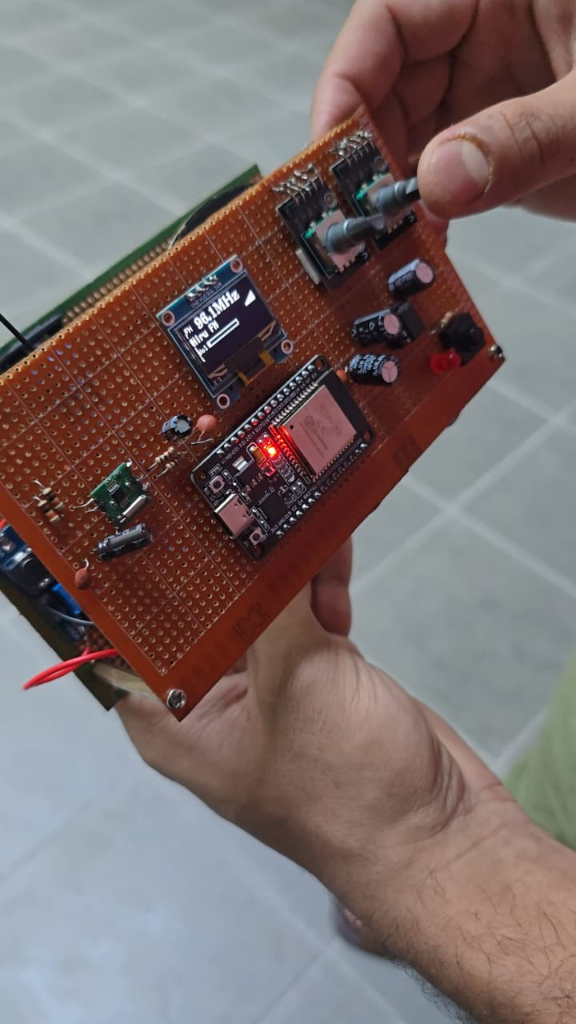
\includegraphics[width=\linewidth]{images/v2_working_1.png}
\end{subfigure}
\hfill
\begin{subfigure}{0.48\textwidth}
\centering
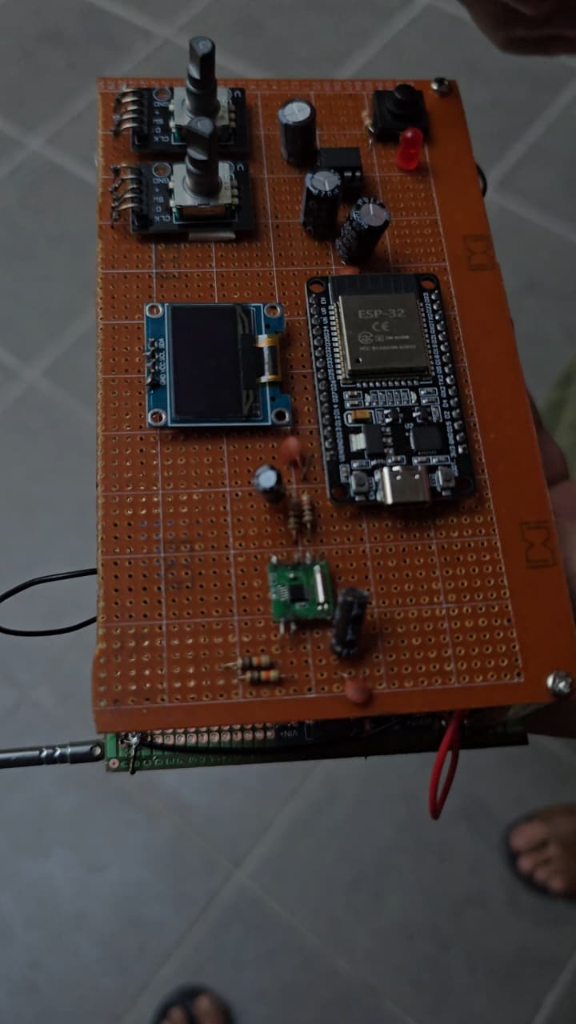
\includegraphics[width=\linewidth]{images/v2_working_2.png}
\end{subfigure}
\caption{Iteration 2 (Dot Board) physical prototype in operation.}
\label{fig:v2-prototype}
\end{figure}


%% ═══════════════════════════════════════════════════════════════════════════════
\subsection{Iteration 3 - Custom PCB Design}
%% ═══════════════════════════════════════════════════════════════════════════════

\textbf{Period:} March 2026.

\medskip\noindent
\hdr{Components}

\begin{itemize}[nosep]
    \item \chip{ATmega328P} (8\,MHz internal oscillator, 3.3\,V)
    \item \chip{RDA5807M} FM receiver
    \item \chip{PAM8403} Class-D stereo amplifier (3\,W$\times$2)
    \item \chip{CH340C} USB-to-UART bridge
    \item \chip{SSD1306} 0.96\textquotedbl{}\ OLED display (128$\times$64)
    \item \chip{TP4056} linear charger + \chip{DW01A}/\chip{FS8205A} battery protection
    \item \chip{HT7333} 3.3\,V LDO regulator
    \item USB-C connector (single port: charging + programming)
    \item Custom 70$\times$50\,mm 2-layer PCB (designed in KiCad~9.0)
\end{itemize}

\medskip\noindent
\hdr{Key Changes from Iteration 2}

\begin{itemize}[nosep]
    \item \chip{ATmega328P} replaces \chip{ESP32} (simpler, cheaper, sufficient)
    \item \chip{PAM8403} Class-D replaces \chip{TDA2822M} (90\,\% efficient, no heatsink)
    \item Single USB-C for both charging and programming
    \item On-board battery protection (\chip{DW01A} + \chip{FS8205A})
    \item Custom PCB designed in KiCad~9.0
\end{itemize}

%% ── Decision callout ──
\begin{calloutdecision}
\textbf{ATmega328P over ESP32}: For the final product, ESP32's WiFi/BT
capabilities were unnecessary overhead.  \chip{ATmega328P} at 3.3\,V /
8\,MHz provides sufficient I/O for I\textsuperscript{2}C + OLED + encoders +
ADC, runs the same Arduino ecosystem, and eliminates level-shifting
complexity.
\end{calloutdecision}

%% ── Design Status callout ──
\begin{calloutnote}[Design Status]
\textbf{Ready for Fabrication}: The Phase~3 design exists in software
(KiCad schematic + PCB layout + comprehensive build guide). It represents the \emph{target architecture}
and provides a complete foundation ready for future fabrication and assembly.
\end{calloutnote}


%% ═══════════════════════════════════════════════════════════════════════════════
\subsection{Iteration Comparison Table}
%% ═══════════════════════════════════════════════════════════════════════════════

\begin{table}[htbp]
\centering
\caption{Comparison of the three design iterations.}
\label{tab:iteration-comparison}
\small
\renewcommand{\arraystretch}{1.25}
\begin{tabularx}{\textwidth}{>{\bfseries}l X X X}
\toprule
\rowcolor{tablehead}
\textcolor{white}{\textsf{Feature}} &
\textcolor{white}{\textsf{Iter.\ 1}} &
\textcolor{white}{\textsf{Iter.\ 2}} &
\textcolor{white}{\textsf{Iter.\ 3}} \\
\midrule
\rowcolor{zebrarow}
MCU         & Arduino UNO          & ESP32                & ATmega328P \\
Radio       & RDA5807M             & RDA5807M             & RDA5807M \\
\rowcolor{zebrarow}
Amplifier   & TDA2822M (SE)        & TDA2822M (BTL)       & PAM8403 (Class-D) \\
Display     & None                 & SH1106 1.3\textquotedbl{} & SSD1306 0.96\textquotedbl{} \\
\rowcolor{zebrarow}
Volume      & Hardware pot         & Software (0--15)     & Software (0--15) \\
Tuning      & Seek buttons         & Rotary encoder       & Rotary encoder \\
\rowcolor{zebrarow}
Power       & USB 5\,V             & 18650 + TP4056       & LiPo + TP4056 + DW01A \\
Audio output& Speaker only         & Speaker only         & Speaker + headphones \\
\rowcolor{zebrarow}
Board       & 15$\times$18\,cm perfboard & 15$\times$9\,cm dot board & 70$\times$50\,mm custom PCB \\
Status      & Built \& working     & Built \& working     & Design completed \\
\bottomrule
\end{tabularx}
\end{table}
